\documentclass[../../main]{subfiles}
\usepackage{graphicx}
\begin{document}
    \section{Practice Modelling Project}
    The purpose of this section is to try to give you some modelling experience in an environment
    that is as close to real world as you can get without actually working on a
    real modelling problem.

    In the system we are working with there are three input variables (or drugs): \bash{S}, \bash{I1} and \bash{I2}.
    The stimulus, \bash{S}, induces phosphorylation and activation of N while the inhibitors \bash{I1}
    and \bash{I2} inhibit G and D respectively.

    I have conducted 4 comprehensive time series experiments which measure the phosphorylated,
    amounts of four key system players: \bash{N}, \bash{G}, \bash{K} and \bash{D}. Each experiment was
    conducted over 2 hours and the system was sampled at 8 time points.
    The data have also been normalised for background noise by subtracting the 0 time point
    from each of the observables. In all experiments, you can assume that the treatments
    are present in saturating concentrations and that this does not change over the
    duration of the experiment.

    Here are the experiments:
    \begin{enumerate}
        \item Stimulation of a cell line with S alone (\bash{S.csv}).
        \item Stimulation of a cell line with S and I1 together (\bash{SI1.csv}).
        \item Stimulation of a cell line with S and I2 together (\bash{SI2.csv}).
        \item Stimulation of a cell line with S with I1 and I2 together (\bash{SI.csv}).
    \end{enumerate}


    \begin{Task}{Building a model from data}
        Use the experimental data you have been given to figure out the
        topology of the network that this data was simulated from.

        However, that does not mean that there are not other topologies that will fit the data.
        Here are some points to consider:
        \begin{itemize}
            \item Firstly, look at the \bash{csv} files and plot your graphs. Use Python to
            write a function to visualise your results. This should go in \bash{data_analysis.py}.
            You should read your data into Python using \bash{pandas.read_csv} then iterate
            over your column names to plot the data using \bash{matplotlib} and \bash{seaborn}.
            The most effective way to visualise would be a to tile the plots from a
            single experiments in a grid, which you can do using \python{plt.subplots}.
            \item Read the experimental protocol. This is essential for determining how to set up your
            simulations.
            \item Draw a wiring diagram(s) for candidate topologies that might fit the data. You're welcome
            to use CellDesigner but remember it can take more time than just drawing a rough diagram
            by hand.
            \item Build the model(s) using antimony. Simulate and plot the data with whichever tool you like.
            \item Use parameter estimation and model selection methods to calibrate your model to the experimental data.
            \item If you have a core hypothesis and some other ideas that you are less certain of, you
            could try using AntimonyCombinations to build combinations of model before configuring them
            for parameter estimation using PyCoTools.
        \end{itemize}

        %        Firstly, there are 10 proteins in this network. They are:
        %        \bash{N}, \bash{pN}, \bash{G}, \bash{pG}, \bash{IG}, \bash{K}, \bash{pK},
        %        \bash{D}, \bash{pD} and \bash{DI}.

    \end{Task}

    \begin{figure}
        \centering
        \begin{minipage}{0.45\textwidth}
            \centering
            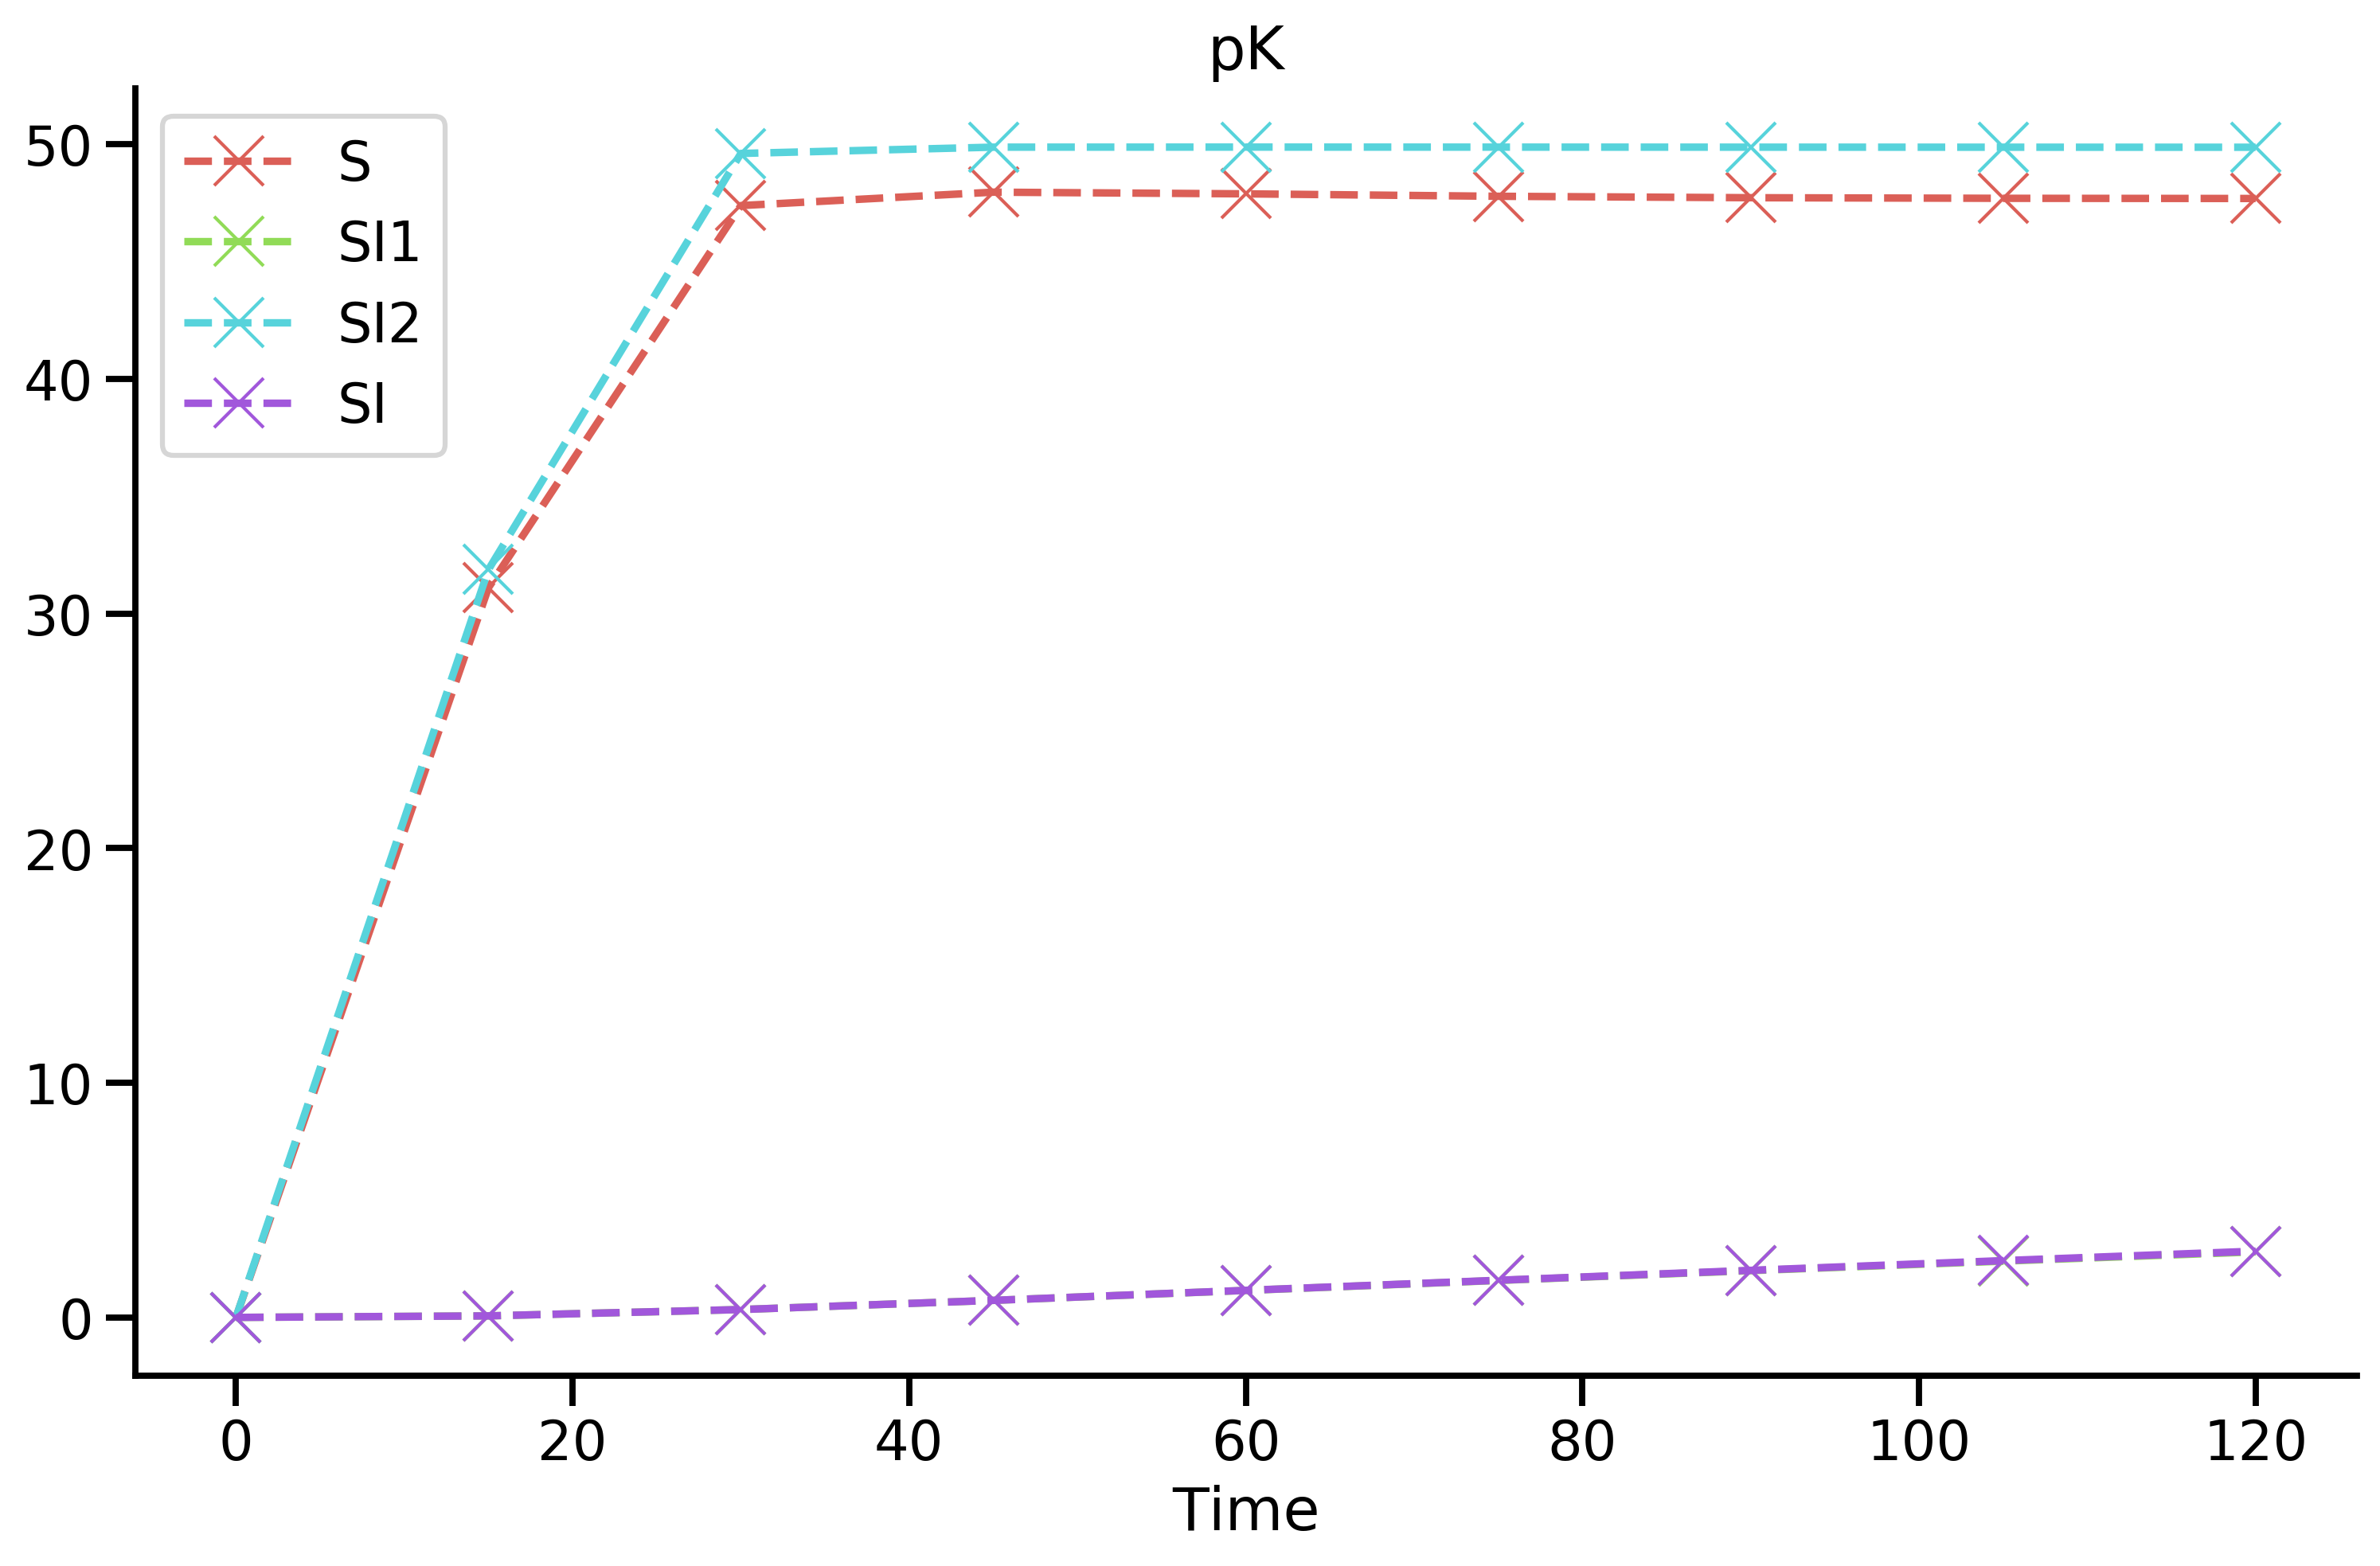
\includegraphics[width=0.9\textwidth]{ODEModels/PracticeProject/pK.png} % first figure itself
            \caption{Measurements of phosphorylated K}
        \end{minipage}\hfill
        \begin{minipage}{0.45\textwidth}
            \centering
            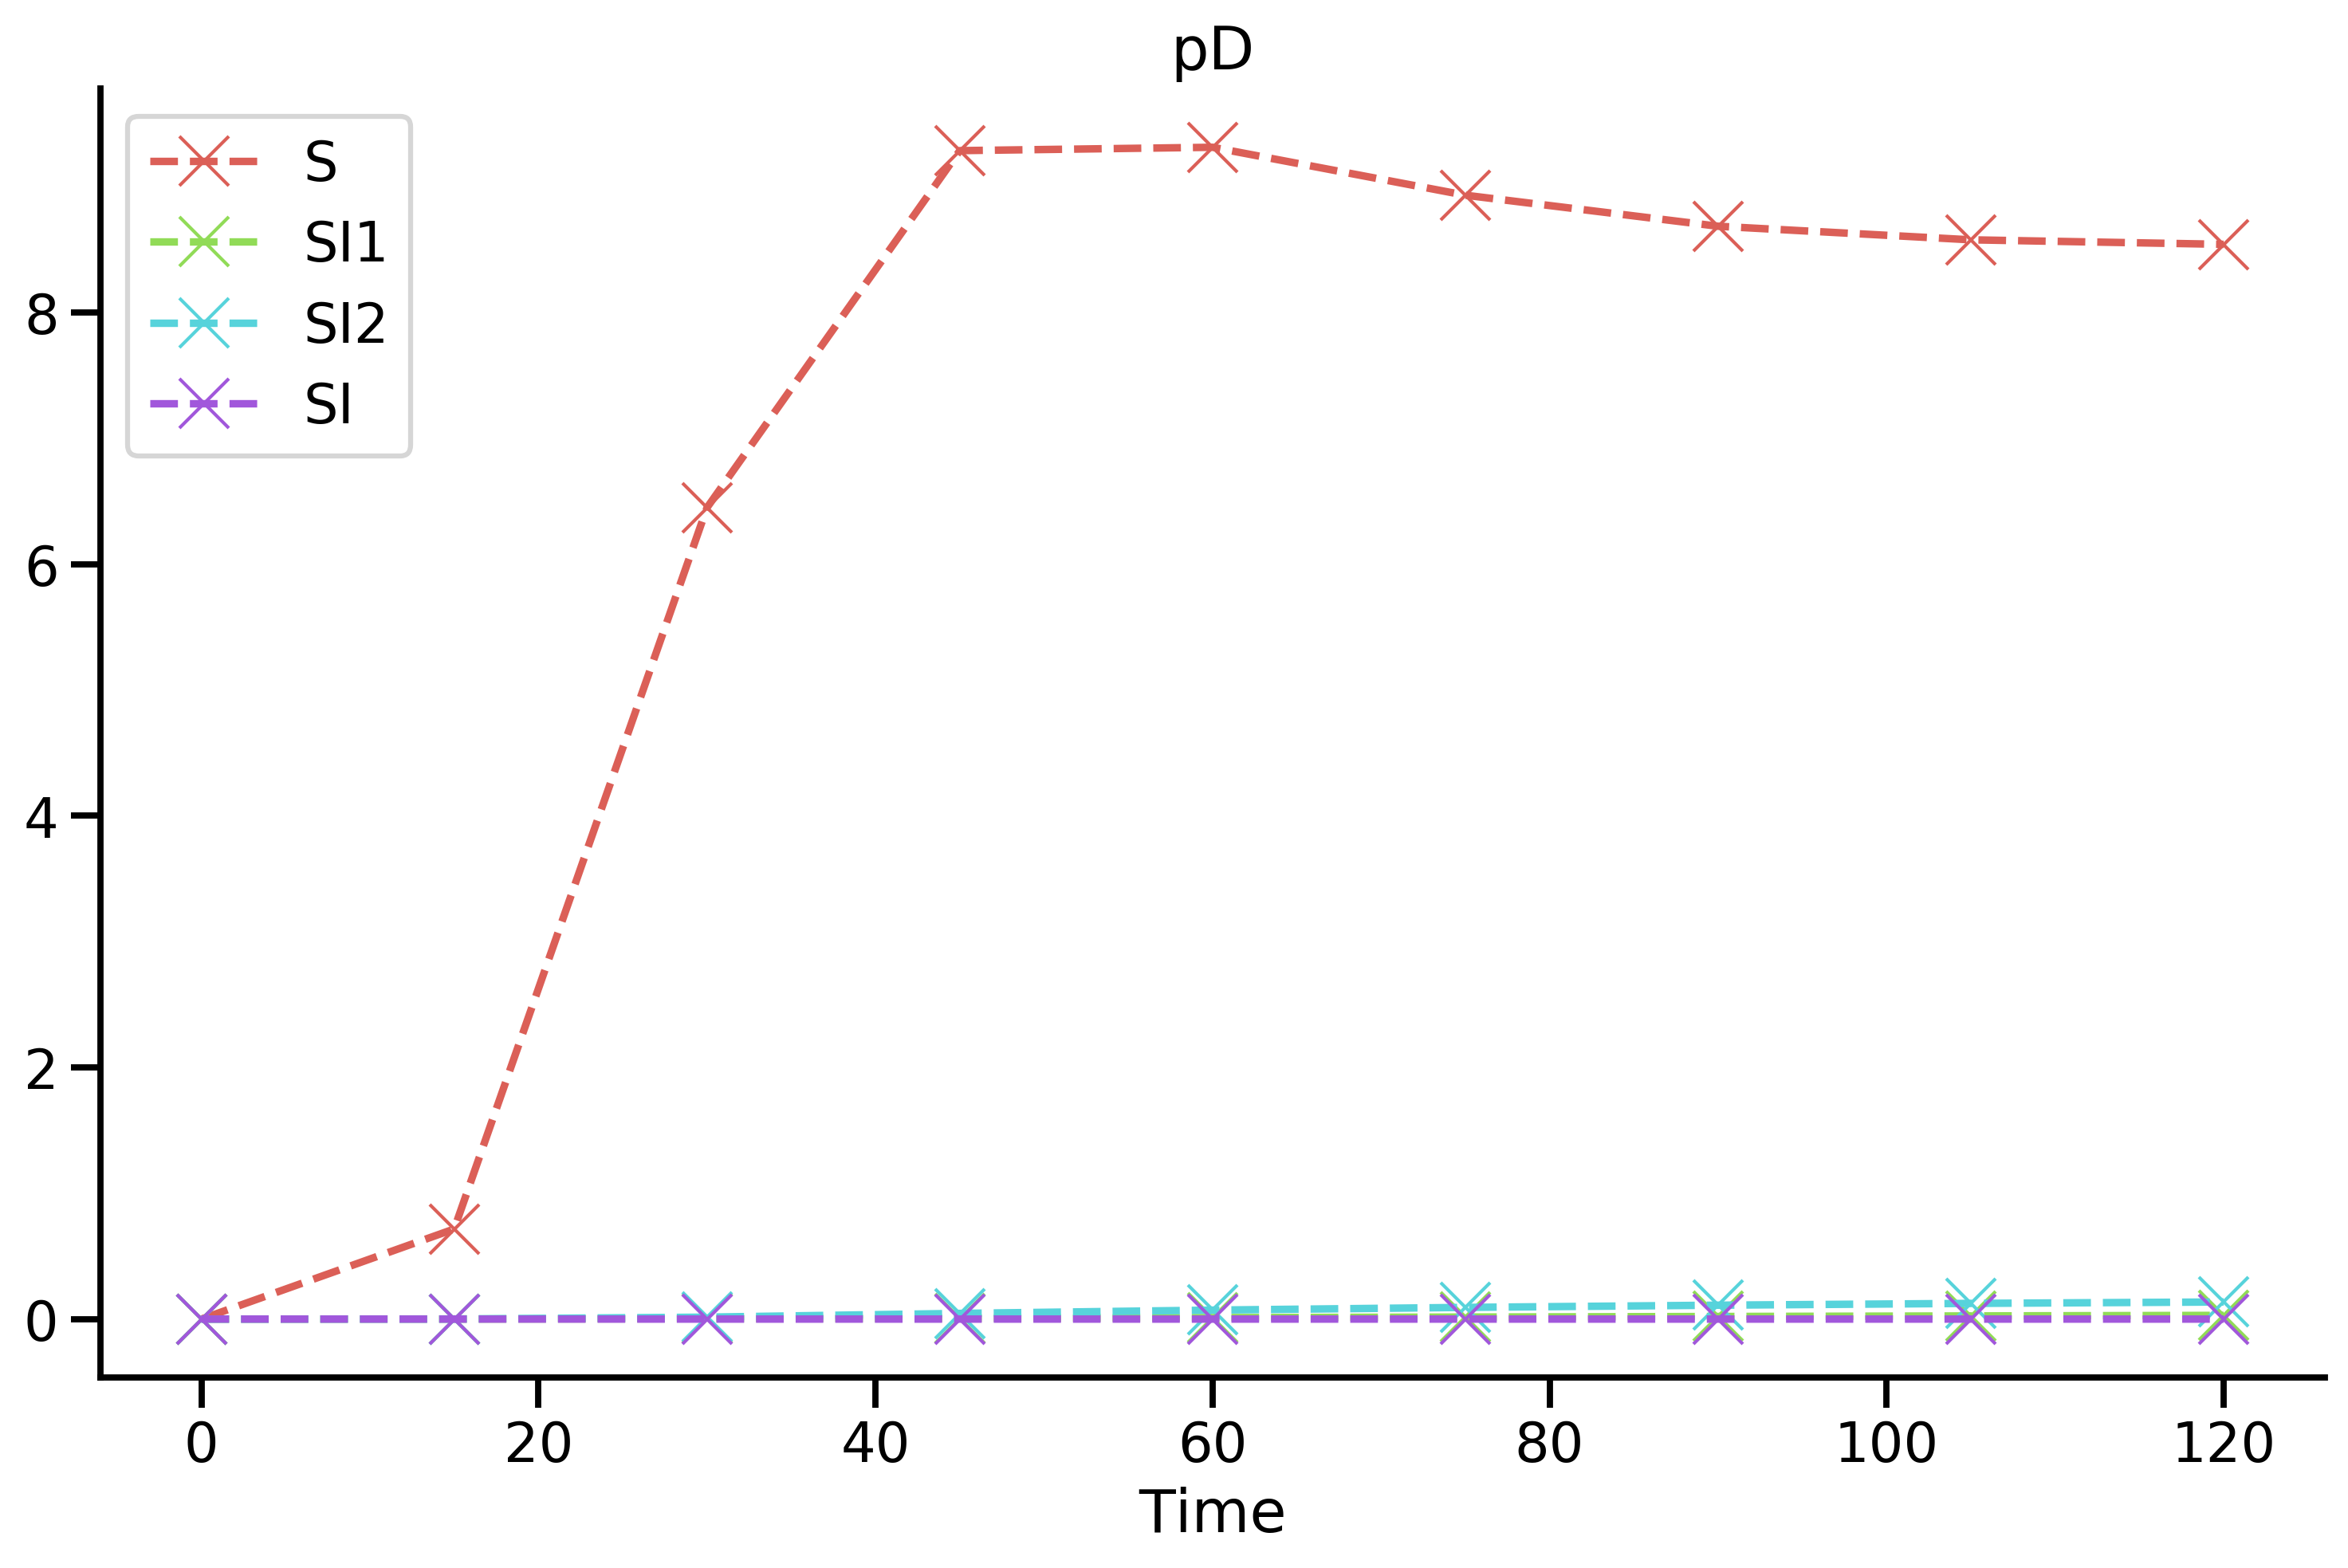
\includegraphics[width=0.9\textwidth]{ODEModels/PracticeProject/pD.png} % second figure itself
            \caption{Measurements of phosphorylated D}
        \end{minipage}\\%
        \begin{minipage}{0.45\textwidth}
            \centering
            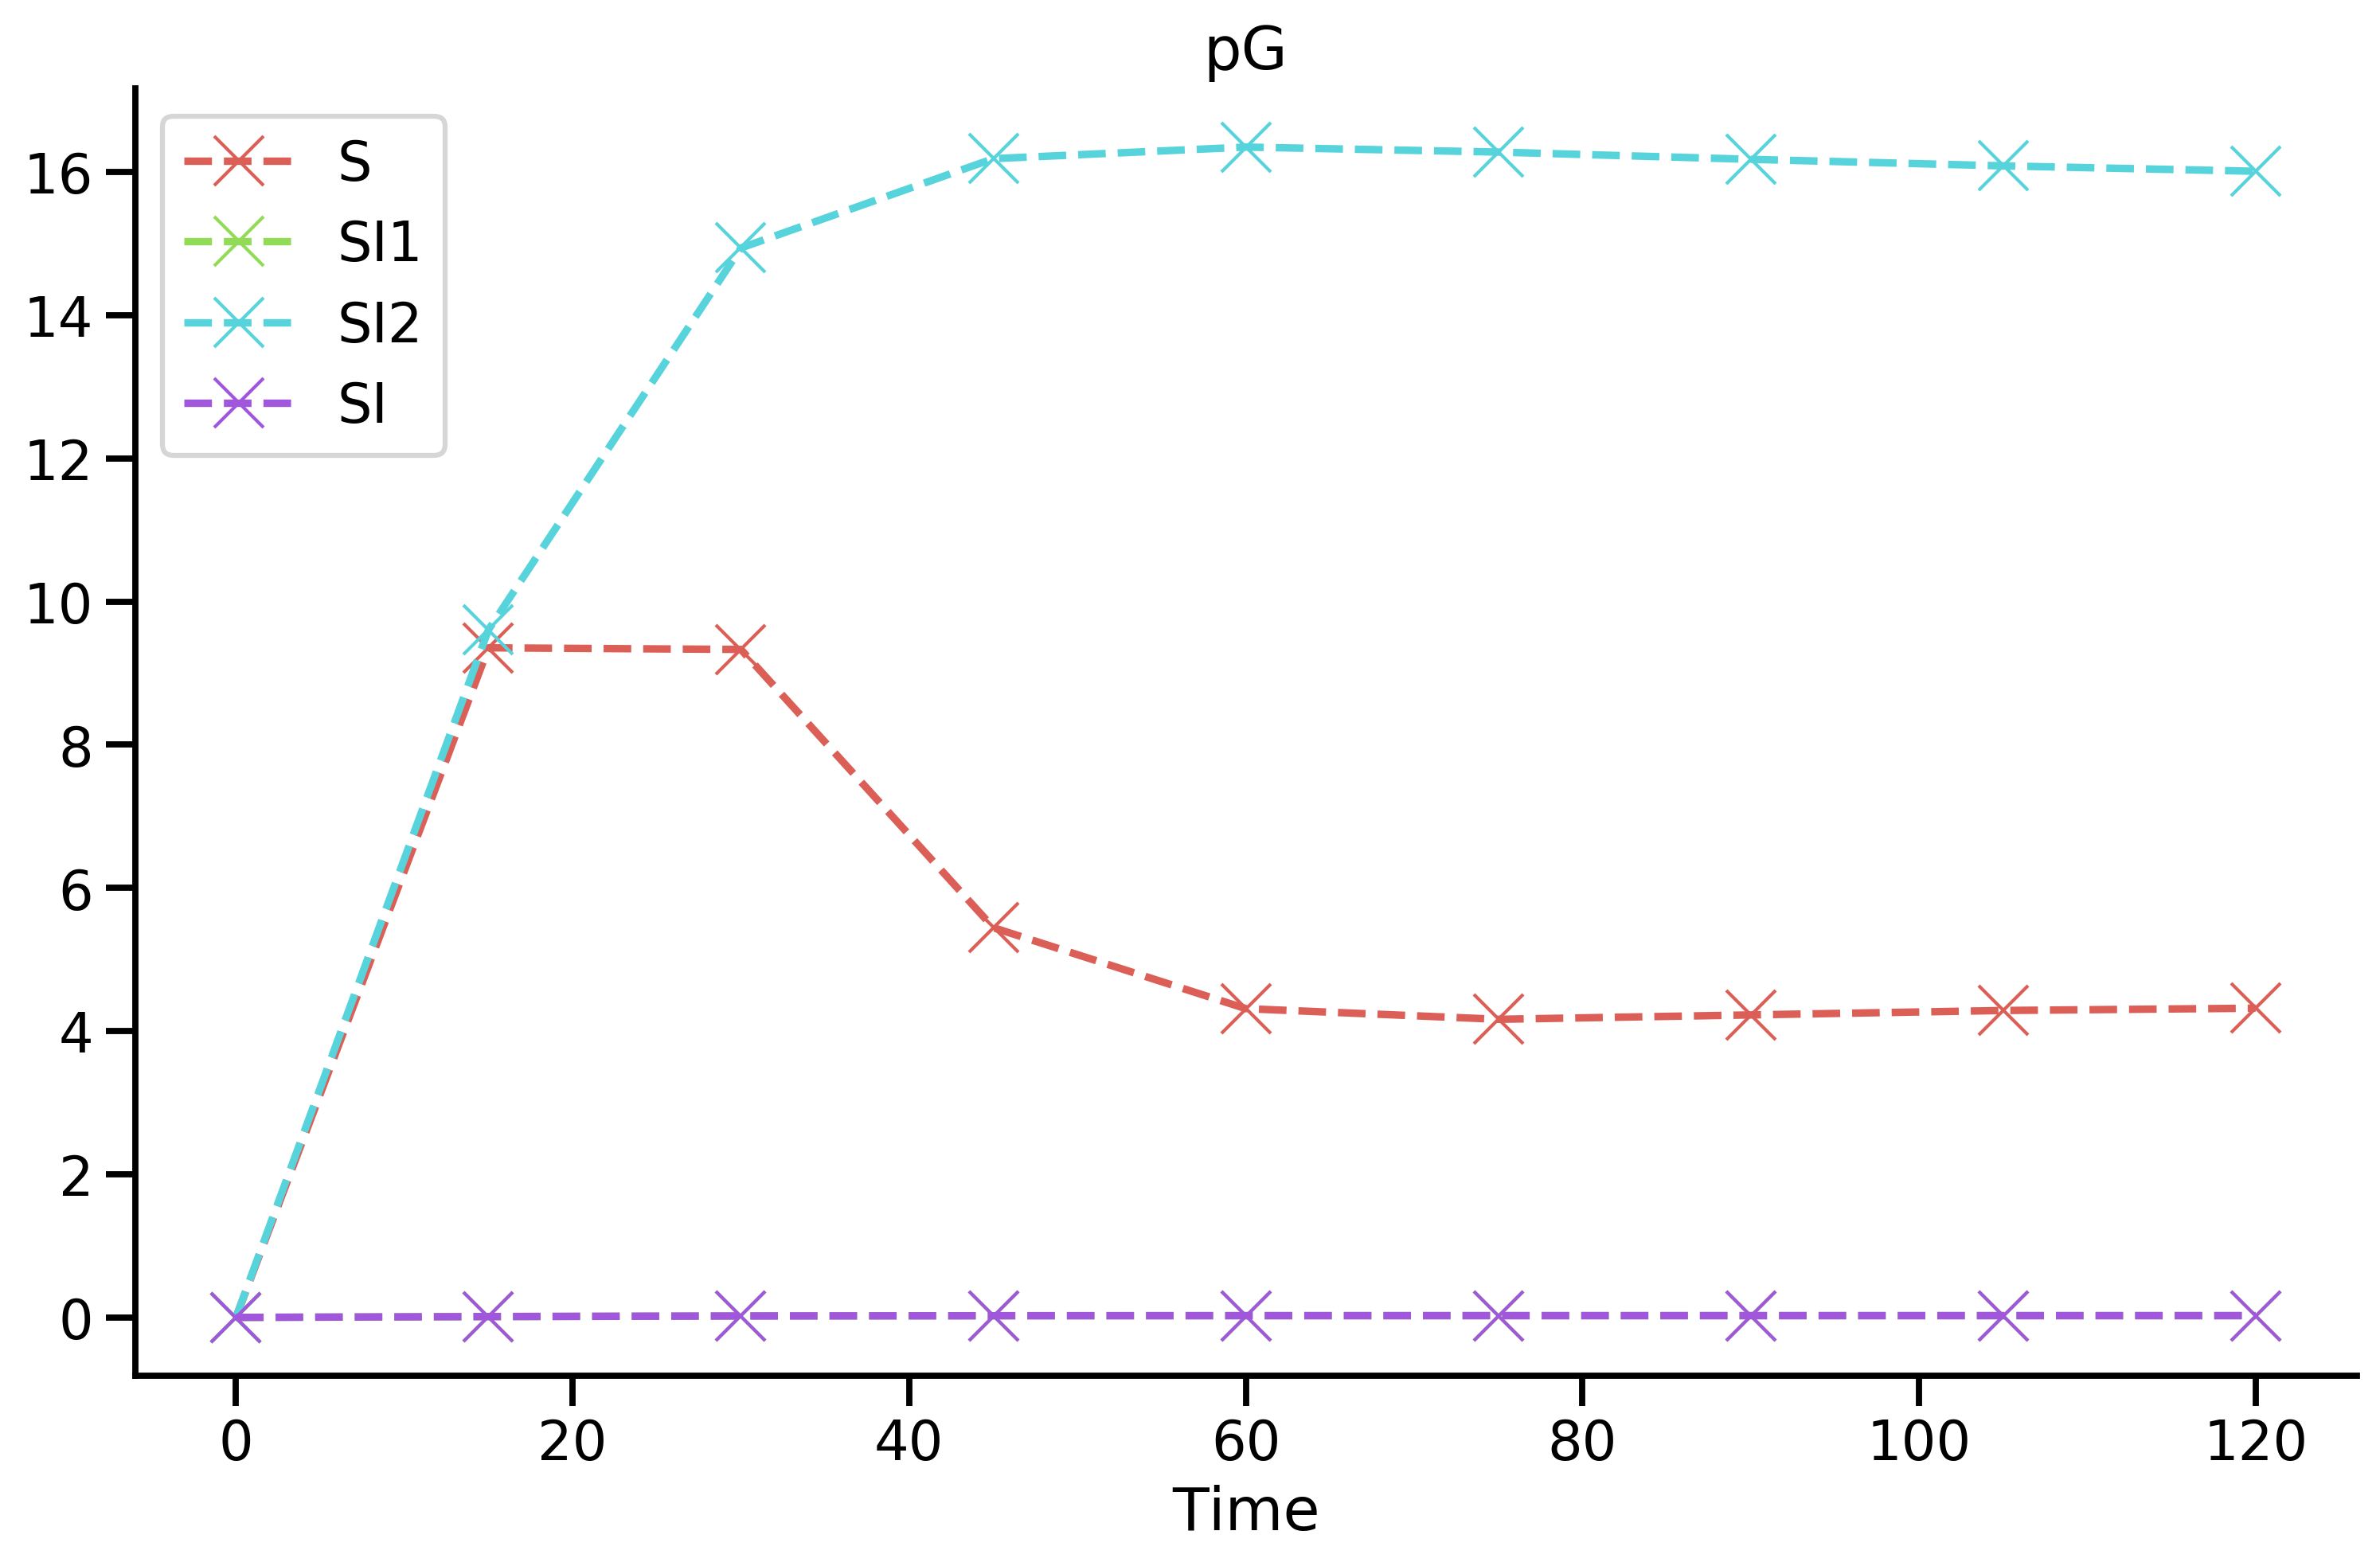
\includegraphics[width=0.9\textwidth]{ODEModels/PracticeProject/pG.png} % second figure itself
            \caption{Measurements of phosphorylated G}
        \end{minipage}\hfill
        \begin{minipage}{0.45\textwidth}
            \centering
            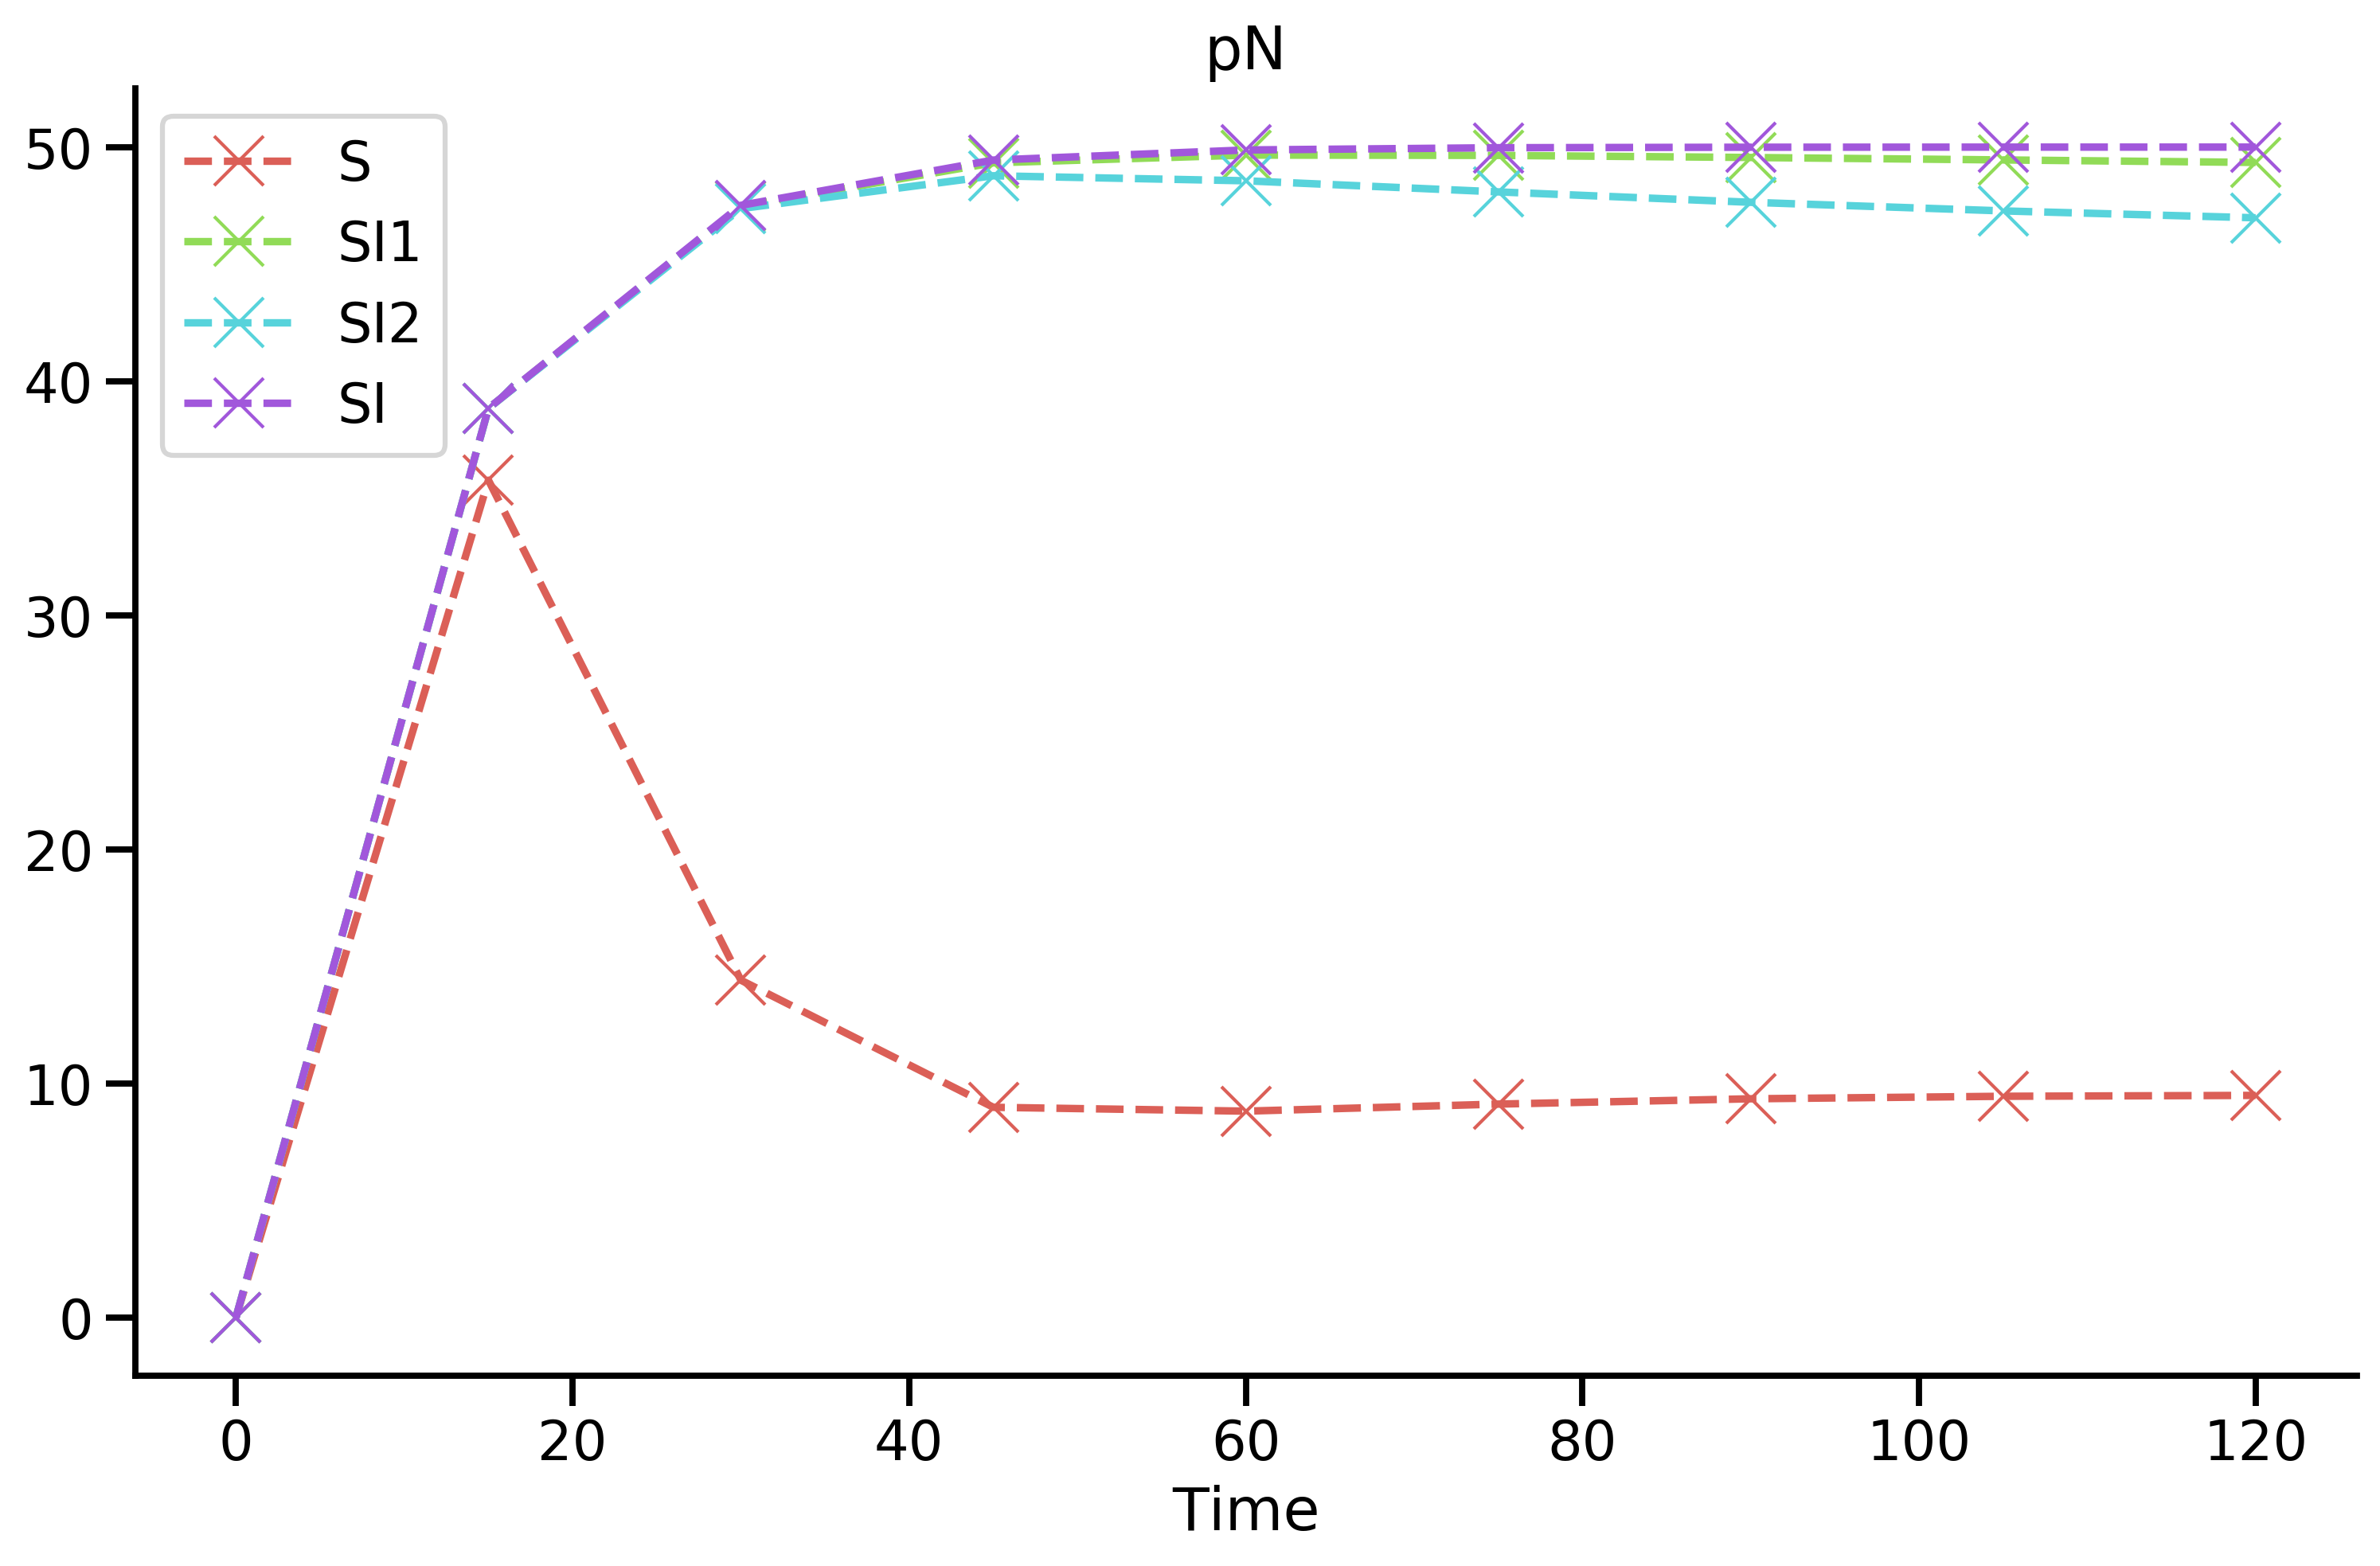
\includegraphics[width=0.9\textwidth]{ODEModels/PracticeProject/pN.png} % second figure itself
            \caption{Measurements of phosphorylated N}
        \end{minipage}
    \end{figure}

\end{document}




















